\documentclass[a4paper]{report}
\usepackage[utf8]{inputenc}
\title{Proposal: Exploring Methods of Procedural Terrain Generation}
\author{Laura Hulley ID: 201277571}
\date{12/11/2020}
\usepackage{url}
\usepackage{float}
\usepackage{wrapfig}
\usepackage{graphicx}
\graphicspath{ {images/} }
\restylefloat{figure}
\renewcommand*{\thesection}{\arabic{section}}
\renewcommand{\thesubsection}{\thesection(\alph{subsection})}

\begin{document}
\maketitle

\section{History and Concepts}
\subsection{}
Genetic Algorithms (GA) and Artificial Neural Networks (ANN) are used to solve a variety of computer science problems. Initially based on biological phenomena, such as evolution and neurons, the techniques are now applied to problems spanning computer science, engineering, economics and more. From predicition \cite{CancerGene}, to optimisation \cite{wiggleAntenna}, these biology-inspired theories are represented algorithmically to solve ground breaking computer science problems. These problems can be biology related (e.g predicting cancer survival rates \cite{CancerGene}), or completely removed from biology (e.g spacecraft antenna development \cite{wiggleAntenna}). The prolific use of these theories within Computer Science and in situations completely removed from their original biological context, warrants the inclusion of these theories as part of Computer Science.

\subsection{}
ANN can be used to solve problems in a range of disciplines including optimisation, prediction, classification, and pattern recognition.
The McCulloch-Pitts neuron was the first proposed computational model of a neuron and first piece of work to be recognised as AI \cite{RussNor}. Many important developments in AI were achieved using ANN as a foundation.

An example of the use of ANN to classify individual handwritten digits can be shown on the MNIST dataset \cite{mnist}. A sample of the 28*28 pixel, greyscale dataset can be seen in figure \ref{fig:mnistSample}

\begin{figure}[H]
    \centering
    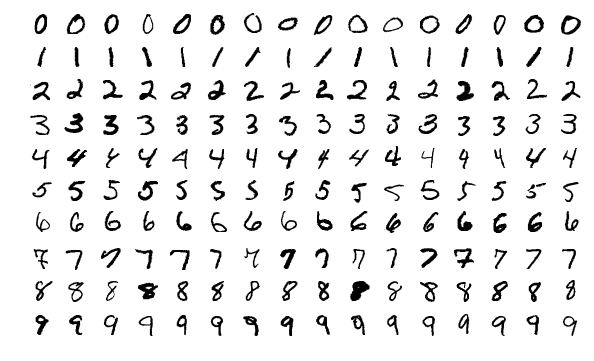
\includegraphics[width=0.8\textwidth]{images/MnistExamples.png}
    \caption{A small sample of the MNIST dataset}
    \label{fig:mnistSample}
\end{figure}

As the images are in greyscale, each pixel in the image can be represented as a numeric greyscale value in an array. These arrays can then form the input to a multi-layered perceptron. Depending on the specific architecture used, the model can ``learn'' what each digit looks like and accurately classify digits it has not seen before. \footnote{This is an extreme oversimplification of the complexity of multilayer perceptrons, even in a seemingly simple application such as this.}

Character recognition such as this has a wide variety of applications, from automatically reading numbers on forms to verifying signature authenticity.

\subsection{}
Genetic algorithms are used to solve optimisation problems spanning a range of disciplines. Inspired by the process of natural selection, they form a subclass of the wider class of evolutionary algorithms. A population of ``chromosomes'' represents a population of candidate solutions to a given optimisation problem. A selection of genetic operators (including mutation, crossover and inversion) are applied to the chromomes and mimic the process that occurs during natural selection.

An example that shows the connection between Genetic Algorithms and their origin in natural selection, can be seen in the following paper \cite{twoLegs} and figure \ref{fig:twoLegsWalk} below.

\begin{figure}[H]
    \centering
    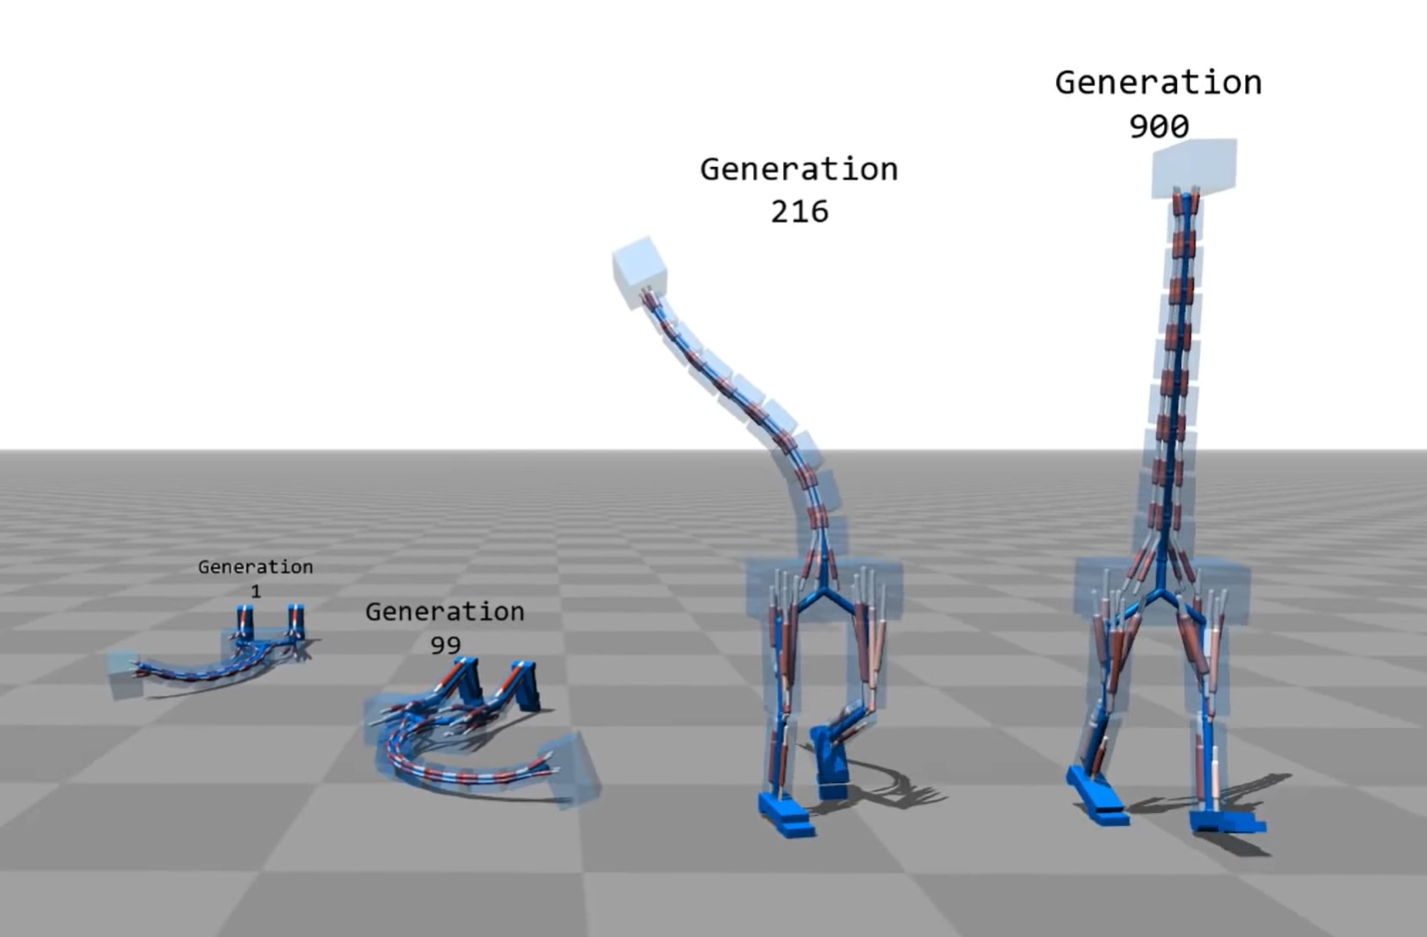
\includegraphics[width=0.8\textwidth]{images/walking.png}
    \caption{Video still, taken from the video at \cite{twoLegsVid}}
    \label{fig:twoLegsWalk}
\end{figure}

In this paper, various optimisation algorithms are used. Most notably in this instance, is the use of the Covariance Matrix Adaptation \cite{CMA}, an evolutionary algorithm. Figure \ref{fig:twoLegsWalk} shows how, over the course of many generations, the chromosomes \footnote{In this case, the choromosomes in question are the values input into the simulated muscles} in a population are optimised towards an objective.

Other applications of genetic algorithms include spacecraft antenna construction \cite{wiggleAntenna}, travelling salesman problem \cite{travellingSales} and boundless others. Despite the wide array of problem disciplines, there are some constraints as to which problems are suitable. For example, problems must have non-differentiable fitness functions and be able to be coded into a string of characters so the genetic operators can be applied.

\subsection{}
\begin{enumerate}
    \renewcommand{\theenumi}{\roman{enumi}}
    \item The OCR system is solving a pattern recognition problem. If the target outputs are listed as classes, it can be seen as a classification problem. At it's simplest form, this can be seen in the many models trained on the MNIST dataset, mentioned in section 1(b), where inputs are classed as a digit between 0 and 9.

    \item There are two main types of OCR algorithm which both take different inputs.

          Matrix matching aims to classify the shapes it identifies in the document as individual characters. It does this using an array value of the shapes and classifying this as a character, based on it's training data - much like MNIST. Any digit from figure \ref{fig:mnistSample} could be an example input, or any individual character on this page. Individual characters such as these are the ideal input however the system could also pick up any other shapes in the document.\footnote{In order to limit the possibility of this occuring, the document will likely undergo pre-processing. Noise can be removed, pages can be aligned and the contrast can be increased to make classification easier.}

          Feature Extraction is another type of OCR algorithm that simplifies the document to a series of features; mainly lines, curves, and intersections. This has many benefits including: the dimensionality of the input is reduced, making the process more efficient; the software can more accurately a variety of font and handwriting styles. Various AI methods can be used to compare the features to those the model is trained on.

    \item There is an intended character/ string for each character/ string being read by the OCR into the system. The training and test data is all labeled. Therefore, this is supervised learning.

          However, there have been recent developments in the area of unsupervised text recognition \cite{unsupervisedTxt}. This paper from the Visual Geometry Group
          at the University of Oxford proposes a method of recognising text in images without labelled traiing data. This combats the time and energy intensive process of manually labelling training data.

          \begin{figure}[H]
              \centering
              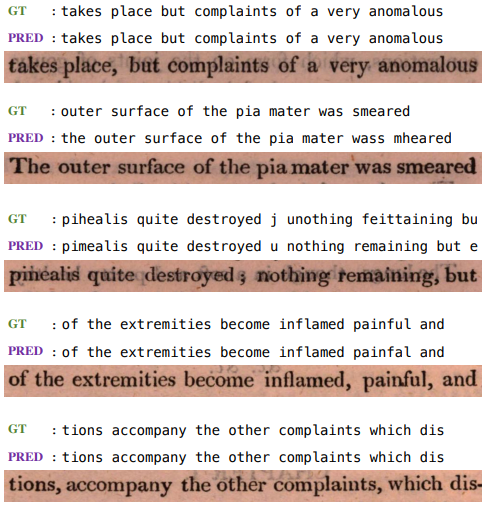
\includegraphics[width=0.5\textwidth]{images/unsprvsdTxt.png}
              \caption{Example results of the model proposed in \cite{unsupervisedTxt}}
              \label{fig:textEg}
          \end{figure}

          As shown in figure \ref{fig:textEg}, there were varying levels of success. Despite this, this is an incredible advancment in text recognition and shows that unsupervised learning may be the future of text recognition. Or a worthy competitor at the very least.

    \item Ignoring the possibility of unsupervised learning, mentioned previously, the network would need to be trained using labelled data. This would likely be in the form of images of characters (handwritten or typed) with their correct label. The NIST dataset (a handwritten character dataset from which MNIST is found) is a good example. Data could also include previously translated and validated documents, any image of text which has an assosciated translation/ label could be used to train the network. The ability for the network to classify characters depends heavily on the training data used. For exammple, a network trained on typed fonts would likely struggle when presented with handwritten characters.
\end{enumerate}

\section{The McCulloch-Pitts neuron}
\subsection{}
See figure \ref{fig:MPflow}, below.

\begin{figure}[H]
    \centering
    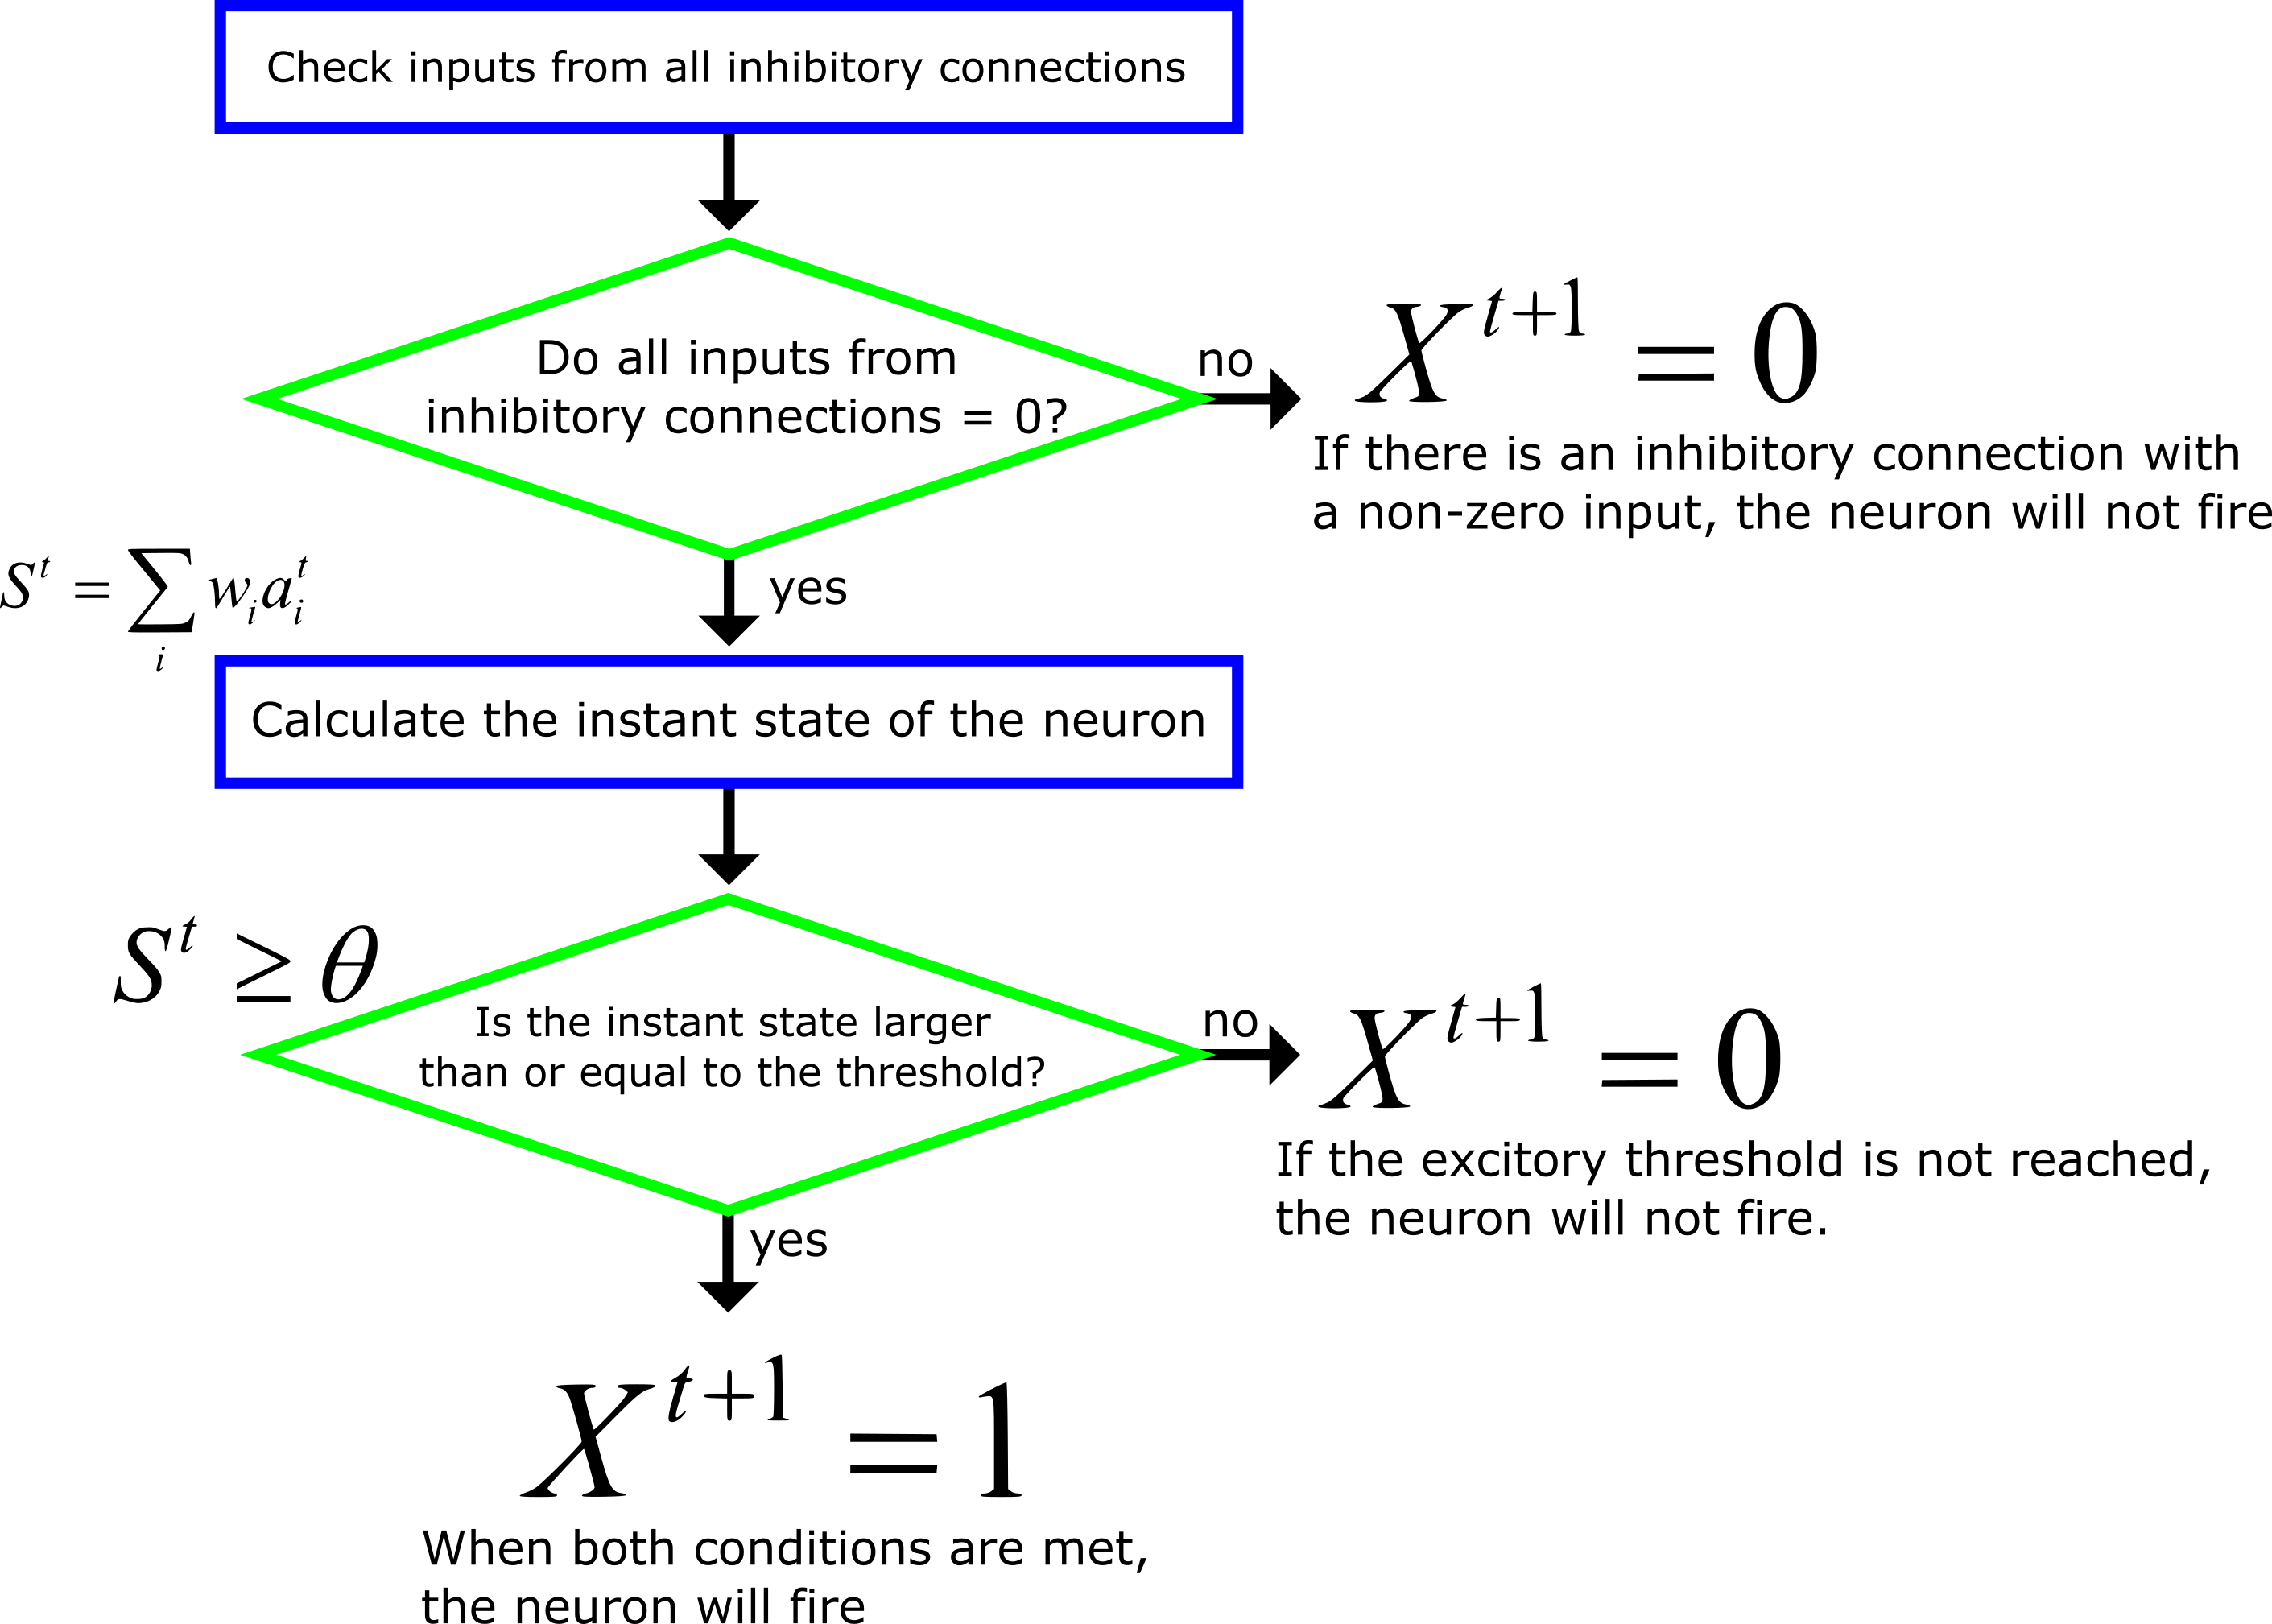
\includegraphics[width=0.9\textwidth]{images/mpFlow.png}
    \caption{A flow chart diagram of an MP neuron where all weights of connections and the neuron threshold are set up in advance.}
    \label{fig:MPflow}
\end{figure}

\subsection{}

Represented in boolean algebra as \(a_1 \vee a_2\), and table form below, the logical OR gate can be represented as an MP-neuron as in figure \ref{fig:or}.

\begin{tabular}{| c | c | c |}
    \hline
    \(a_1\) & \(a_2\) & ``\(OR\)'' \\ [0.5ex]
    \hline\hline
    1       & 1       & 1          \\
    \hline
    1       & 0       & 1          \\
    \hline
    0       & 1       & 1          \\
    \hline
    0       & 0       & 0          \\ [1ex]
    \hline
\end{tabular}
\linebreak
\linebreak

This table shows all possible outputs of the OR gate depending on all possible input values of \(a_1\) and \(a_2\). If either of \(a_1\) and \(a_2\) is ``true'' (has an input of 1), then the neuron will fire (\(X = 1\)).

\begin{figure}[H]
    \centering
    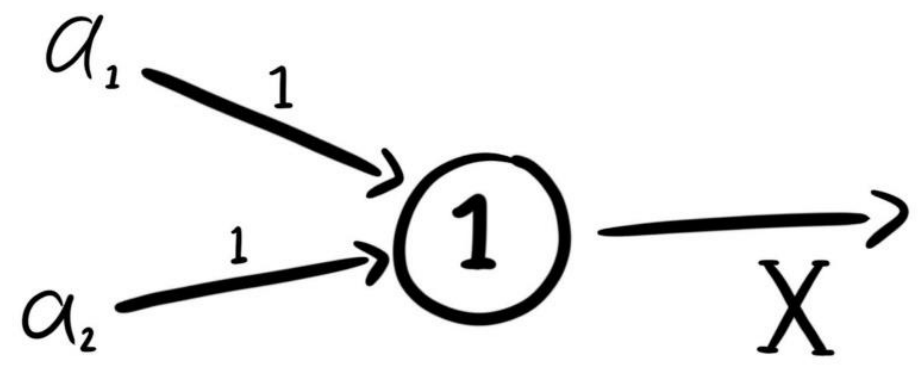
\includegraphics[width=0.7\textwidth]{images/or.png}
    \caption{A diagram of an MP-neuron realisation of an
        “OR” logical gate}
    \label{fig:or}
\end{figure}

For this OR gate, the excitation threshold (\(\theta\)) must be \(0 < \theta \leq 1\). The value of 1 is chosen in figure \ref{fig:or}, but any value within the given range would be sufficient. This inequlity can be proven to be correct by analysing the output for each possible value of \(a_i\) (assuming the weights remain at 1).

The following values of \(a_i\) should fire the neuron (\(X = 1\)) when the excitation threshold is 1 (\(\theta = 1\)) as at least one of \(a_1\) and \(a_2\) is always true (equal to 1).

\(a_1 = 1, a_2 = 1 \Rightarrow  a_1 + a_2 = 1 + 1 = 2, 2 \geq \theta \Rightarrow X = 1\)

\(a_1 = 1, a_2 = 0 \Rightarrow  a_1 + a_2 = 1 + 0 = 1, 1 \geq \theta \Rightarrow X = 1\)

\(a_1 = 0, a_2 = 1 \Rightarrow  a_1 + a_2 = 0 + 1 = 1, 1 \geq \theta \Rightarrow X = 1\)

Conversley, if neither of \(a_1\) and \(a_2\) are true then excitation threshold should not be reached and the neuron will not fire.

\(a_1 = 0, a_2 = 0 \Rightarrow  a_1 + a_2 = 0 + 0 = 0, 0 < \theta \Rightarrow X = 0\)

The above functions show that the inequality of the excitation threshold must be \(0 < \theta \leq 1\).

\subsection{}

Represented in boolean algebra as \(\neg a_1\), and table form below, the logical OR gate can be represented as an MP-neuron as in figure \ref{fig:not}.

\begin{tabular}{| c | c |}
    \hline
    \(a_1\) & ``\(NOT\)'' \\ [0.5ex]
    \hline\hline
    1       & 0           \\
    \hline
    0       & 1           \\ [1ex]
    \hline
\end{tabular}
\linebreak
\linebreak

This table shows all possible outputs of the NOT gate depending on all possible input values of \(a_1\).
\begin{figure}[H]
    \centering
    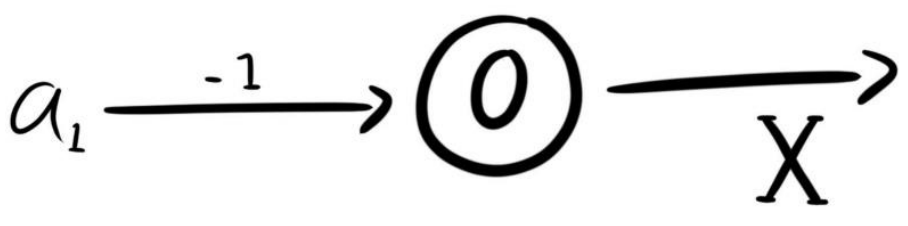
\includegraphics[width=0.7\textwidth]{images/not.png}
    \caption{A diagram of an MP-neuron realisation of a
        “NOT” logical gate}
    \label{fig:not}
\end{figure}

For this NOT gate, the excitation threshold (\(\theta\)), must be \(\theta = 0\). This threshold value can be proven to be correct by analysing the output for each possible value of \(a_1\).

If \(a_1\) is true (\(a_1 = 1\)), it causes in input from an inhibitory connection, therefore the neuron will not fire. If \(a_1\) is false (\(a_1 = 0\)), then the threshold is met as \(0 \geq \theta\). The neuron will fire.

\subsection{}
The first neuron is an OR gate. Since both \(a_1\) and \(a_2\) are 0, it will not as the threshold of 1 is not met. This can also be seen in table format in question 2(b). This is followed by a NOT gate. Since the first neuron has not fired (providing an input of 0), this neuron will fire as the threshold of 0 is met. This logic can be seen in the NOT gate in question 2(c). As this is the final gate, and it has fired, the output is \(X = 1\) (The neuron fires).

These answers can also be found by following the flow chart shown in part 2(a), as seen in figure \ref{fig:mpPath}

\begin{figure}[H]
    \centering
    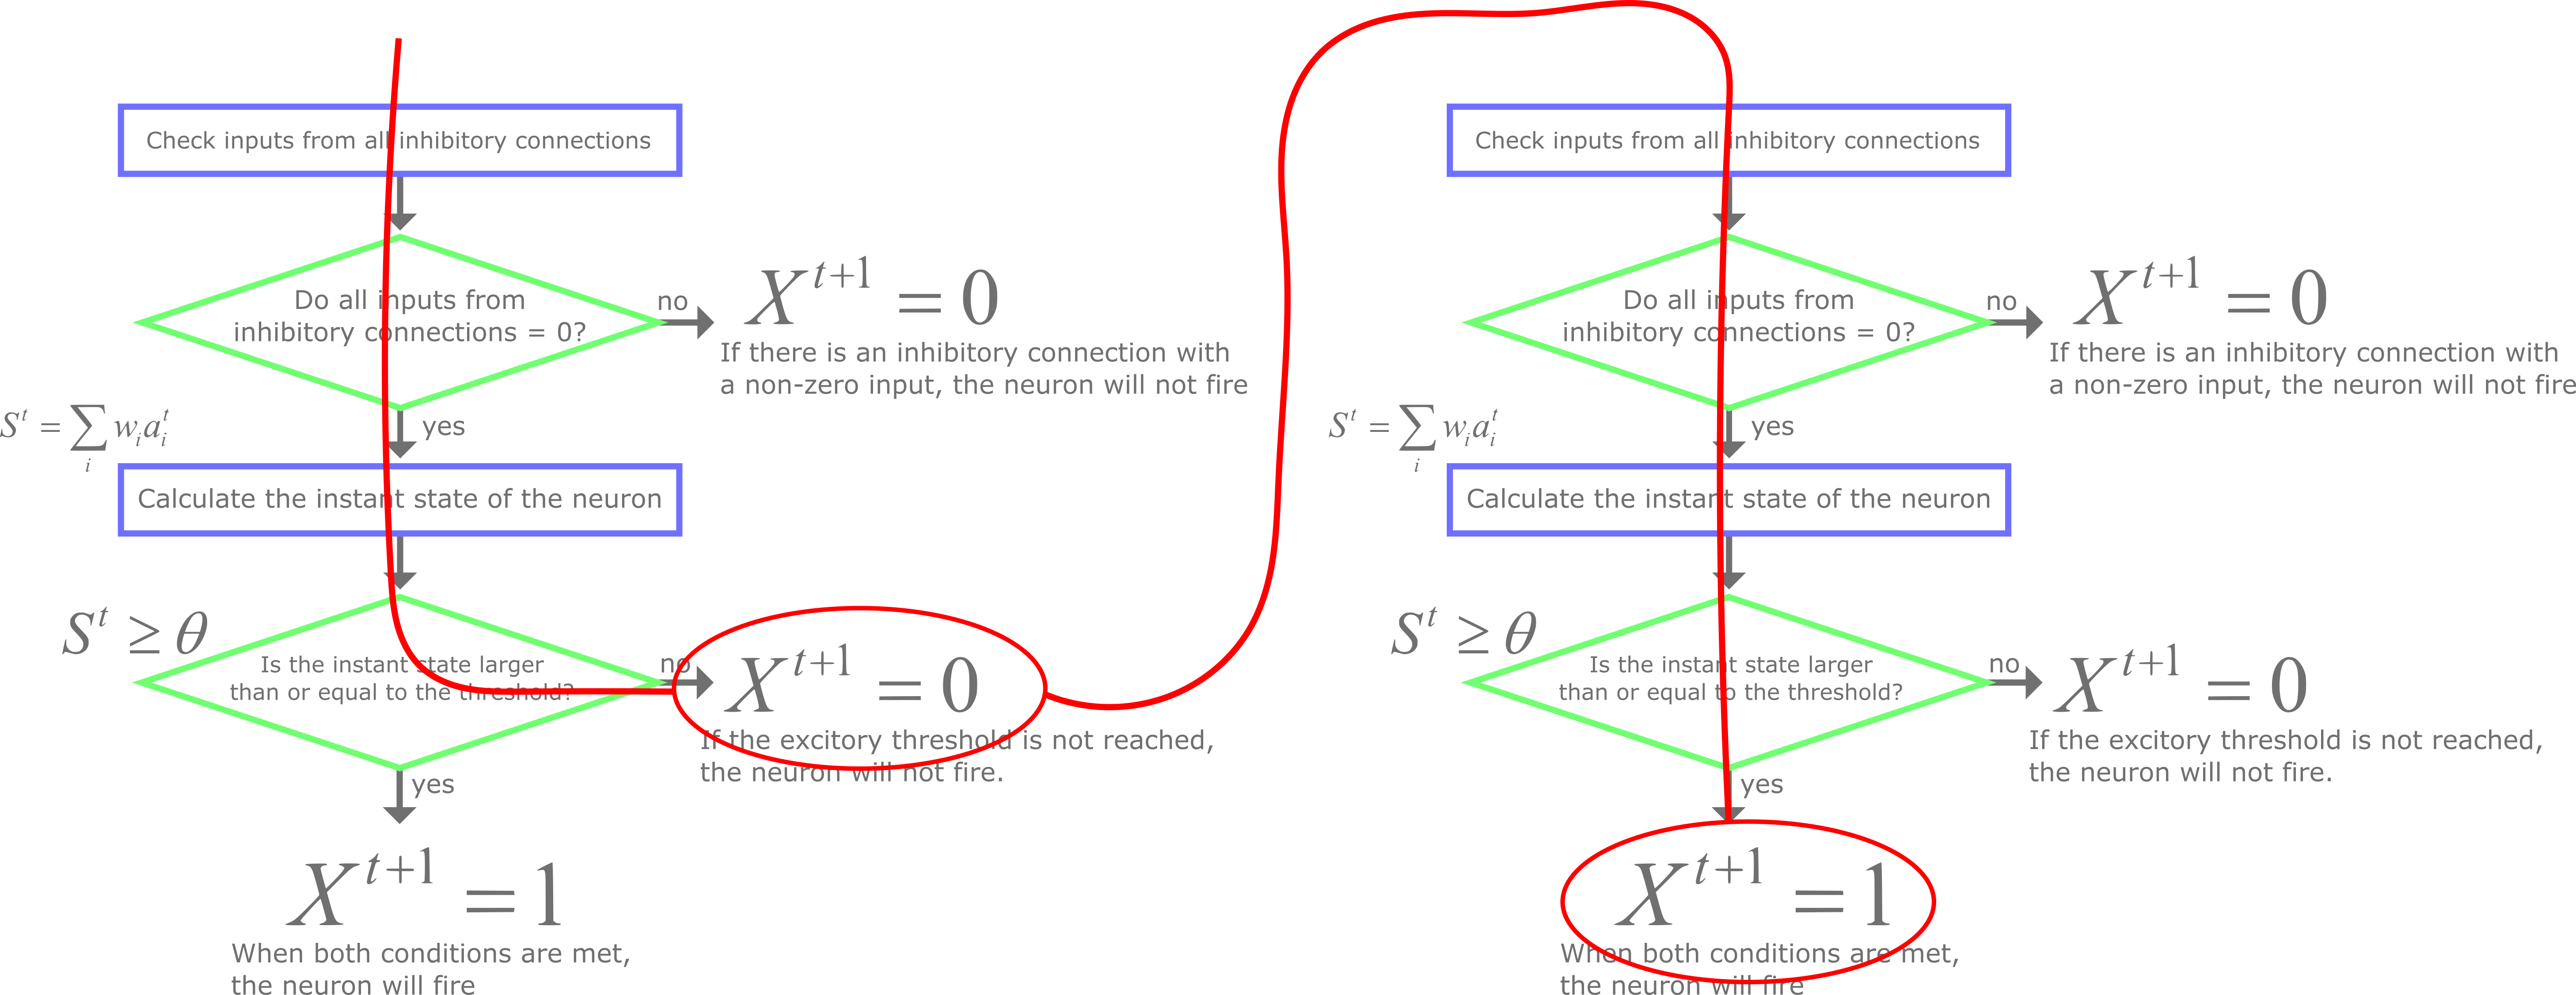
\includegraphics[width=0.8\textwidth]{images/mpRoute.png}
    \caption{The route taken through the flow chat for the network in question 2(d)}
    \label{fig:mpPath}
\end{figure}

\subsection{}
Figure \ref{fig:mem} shows the MP-neuron representation of a memory cell. A memory cell, such as this, can be formed by closing a neuron in a feedback loop. To initialise this cell, an excitory input (\(a_1\) in this case) is fired. This causes the value of 1 to cycle the loop (repeatedly fire the neuron), essentially storing it in the cell's memory. Even if \(a_1\) were to fire again, the loop would still be constant at 1. That is, until the inhibitory connection fires. \(a_2\) firing would cause the neuron to not fire, therefore breaking the cycle.
\begin{figure}[H]
    \centering
    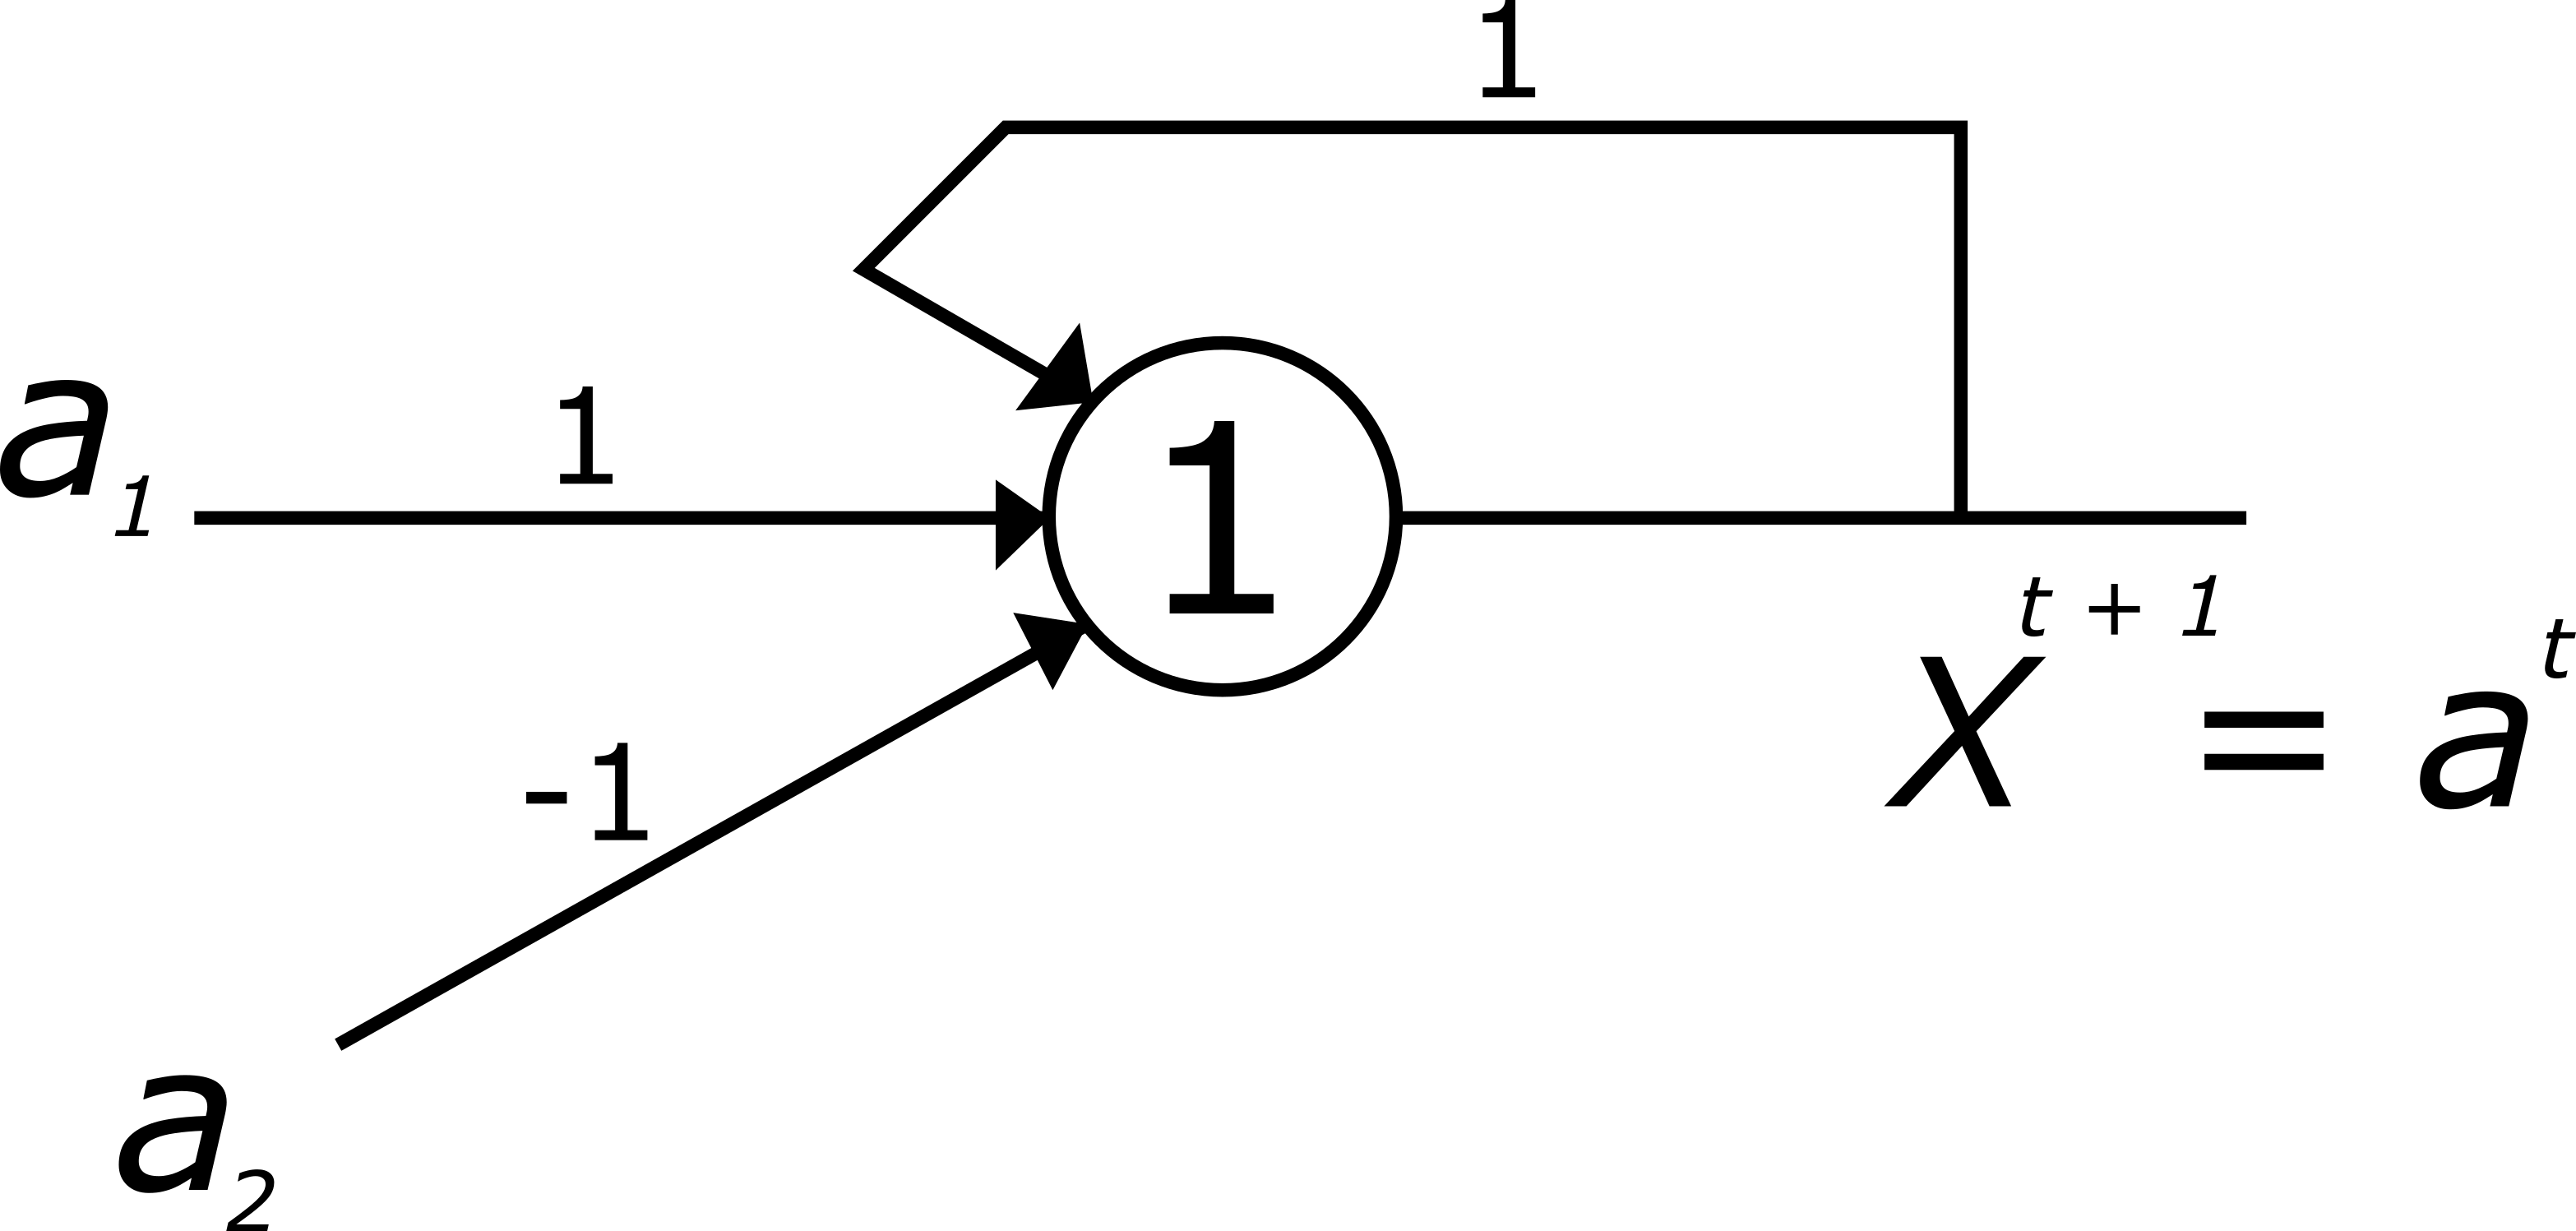
\includegraphics[width=0.8\textwidth]{images/memory.png}
    \caption{An MP-neuron representation of a memory cell}
    \label{fig:mem}
\end{figure}

\section{Learning rules of the Artificial Neural Networks. Hebb’s Rule.}
\subsection{}

\renewcommand\bibname{References}
\bibliographystyle{IEEEtran}
\bibliography{refs}
\end{document}